\hypertarget{a00018}{}\section{Algorytm1.\+cpp File Reference}
\label{a00018}\index{Algorytm1.\+cpp@{Algorytm1.\+cpp}}


Metody klasy \hyperlink{a00002}{Algorytm1}.  


{\ttfamily \#include \char`\"{}Algorytm1.\+hh\char`\"{}}\\*
Include dependency graph for Algorytm1.\+cpp\+:
\nopagebreak
\begin{figure}[H]
\begin{center}
\leavevmode
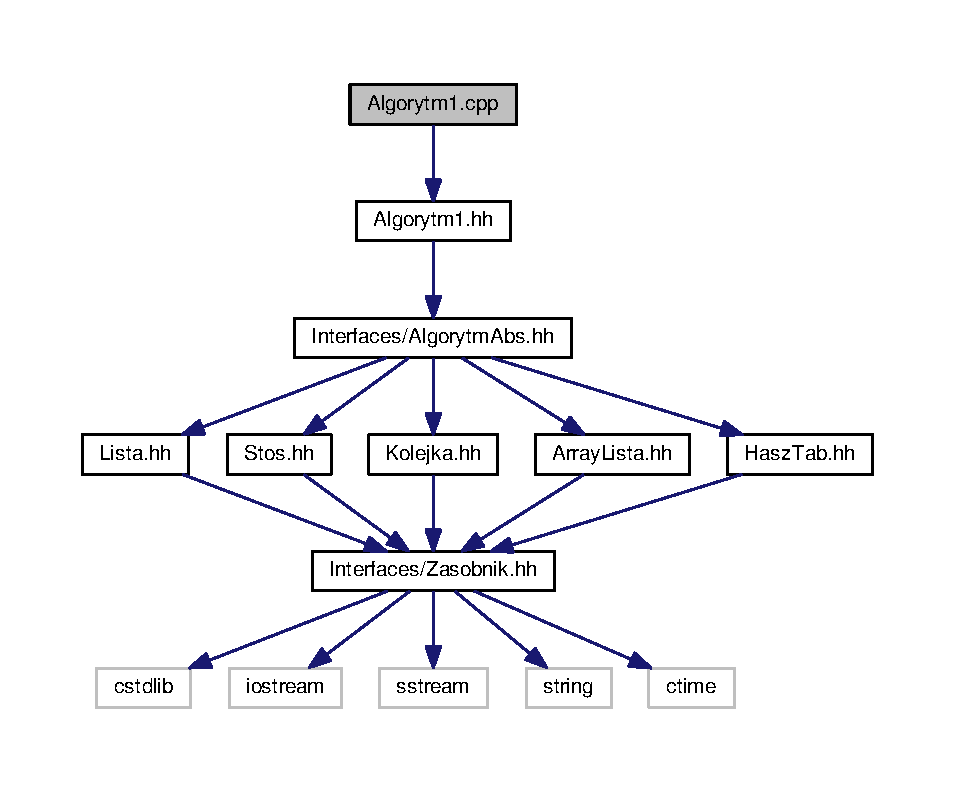
\includegraphics[width=350pt]{a00053}
\end{center}
\end{figure}


\subsection{Detailed Description}
Metody klasy \hyperlink{a00002}{Algorytm1}. 

Plik zawiera metody klasy \hyperlink{a00002}{Algorytm1}. 